\documentclass[pdflatex,sn-mathphys-ay]{sn-jnl}

\usepackage{graphicx}
\usepackage{booktabs}
\usepackage{amsmath,amssymb,amsfonts}
\usepackage{amsthm}
\usepackage{mathrsfs}
\usepackage[title]{appendix}
\usepackage{xcolor}
\usepackage{textcomp}
\usepackage{manyfoot}
\usepackage{listings}
\usepackage{float}
\usepackage{pgfplots}
\pgfplotsset{compat=1.18}
\usepackage{tikz}
\usetikzlibrary{shapes.geometric, arrows.meta, positioning, fit, backgrounds, calc}

% We load algorithm2e and set it up as done in the baseline RESEARCH_PAPER.tex
\usepackage[ruled,lined,linesnumbered]{algorithm2e}
\SetAlgoNlRelativeSize{-1}
\SetAlgoSkip{medskip}

% Map Elsevier template custom column types to match sn-jnl
\usepackage{array}
\newcolumntype{L}{@{\extracolsep{\fill}}l}
\newcolumntype{R}{@{\extracolsep{\fill}}r}
\newcolumntype{C}{@{\extracolsep{\fill}}c}
\newcolumntype{P}[1]{>{\raggedright\arraybackslash}p{#1}}
\def\tblwidth{\textwidth}

\raggedbottom

\begin{document}

\title[GEE-LLM: Grounded GEE Code Gen and Scientific Interpretation]{GEE-LLM: Grounded Google Earth Engine Code Generation and Scientific Interpretation for Geospatial Decision Support}

% Author blocks omitted for double-blind peer review

\abstract{Satellite Earth observation generates an extraordinary volume of environmental data, yet translating that data into actionable geospatial insight remains a persistent barrier for domain scientists, planners, and policy-makers who lack programming expertise in cloud-based spatial platforms such as Google Earth Engine (GEE). A hydrologist tracking watershed vegetation decline, an urban planner assessing land surface temperature trends, or a forest manager monitoring deforestation does not require a raw numerical array --- they require a clear, scientifically grounded explanation of what the data reveals and what patterns are ecologically significant. Existing large language model (LLM) approaches to geospatial automation address only one part of this challenge: they generate code, but either fail to produce scripts that execute correctly on GEE's client-server lazy-evaluation architecture, or when they do succeed, deliver numeric outputs that leave the final interpretive burden entirely with the user. We introduce GEE-LLM, a lightweight, compute-agnostic framework that closes this complete loop from natural language query to decision-ready geospatial intelligence. A first LLM pass generates and self-corrects executable GEE Python code through a sandboxed execution engine, a physical boundary validation layer, and a TF-IDF lexical template retrieval module, all running on commodity CPU hardware without GPU infrastructure. A second-pass LLM then receives only the execution-validated numeric result and produces a grounded natural-language scientific interpretation, translating verified satellite statistics into human-readable environmental insight without access to raw imagery or source code. Evaluated against a 100-query benchmark spanning the diverse ecological zones of the Indian subcontinent --- from Himalayan glaciated regions to the arid Thar Desert and monsoon-affected coastal zones --- the framework raises execution success rates from 12.0\% and 17.0\% (zero-shot baselines for Cohere Command-A and Groq Llama-3.3-70B respectively) to 44.0\% and 45.0\% under the full system. McNemar's tests confirm these gains are highly statistically significant ($p < 0.001$), with odds ratios reaching 15.0. The grounded interpretation stage produces scientifically descriptive trend narratives verified against the underlying histogram distributions, demonstrating that GEE-LLM delivers not merely executable code, but complete, trustworthy geospatial decision support.}

\keywords{Google Earth Engine, Large Language Models, Geospatial Decision Support, Grounded Code Generation, Scientific Interpretation}

\maketitle

\section{Introduction}\label{sec:intro}

The volume of satellite Earth observation data available to environmental scientists, planners, and resource managers has grown to an unprecedented scale. Yet for the practitioner who needs to answer a concrete operational question --- whether a reservoir's catchment area is losing vegetation cover, whether monsoon flooding in a delta is worsening year-on-year, whether an urban heat island is intensifying over a growing metropolitan region --- raw access to this data provides little immediate value. What is needed is not simply a data archive, but a system that can receive a natural-language question, retrieve and compute the relevant satellite statistics, and translate those statistics into a clear, scientifically grounded interpretation that supports a real decision. Existing tools do not deliver this complete chain. Geographic information platforms require programming expertise. Large language models (LLMs) capable of generating the necessary code frequently produce scripts that fail to execute correctly. And even when execution succeeds, the numeric output is handed back to the user without any interpretive context, leaving the final and most cognitively demanding step of the analysis entirely unassisted.

Satellite remote sensing is indispensable for global environmental science, enabling researchers to monitor ecosystems, climate dynamics, and land cover at scale. Cloud-based Geographic Information Systems, particularly Google Earth Engine (GEE), have lowered hardware barriers by centralizing petabyte-scale archives and offloading processing to distributed server-side clusters \citep{Gorelick2017, Amani2020}. Google Earth Engine has also enabled integrated multi-sensor remote sensing studies by combining optical, thermal, atmospheric, and nighttime satellite observations within a unified cloud-based analytical framework \citep{Kasana2026}. However, utilizing GEE demands specialized expertise in client-server programming models. Because GEE builds deferred computational graphs for remote evaluation, client-side libraries do not execute operations locally. Developers must define a Directed Acyclic Graph (DAG) using proxy variables. A common mistake is writing standard local loops or primitive arithmetic on these proxies, which causes backend compilation crashes when sent to the server.

This lazy-evaluation mismatch is exacerbated by sensor constraints. Calculating spectral indices requires exact band names, scaling factors, and resolution limits. For instance, Sentinel-2 uses bands \texttt{B8} and \texttt{B4} for infrared and red reflectance, whereas Landsat 8 requires \texttt{SR\_B5} and \texttt{SR\_B4}. Furthermore, spatial reductions require explicit scale parameters; running a regional reducer over large boundaries without setting an appropriate pixel scale causes the GEE scheduler to default to native resolution, attempting to compute millions of pixels at once and triggering memory limit exceptions.

Large language models (LLMs) often struggle with these constraints, routinely producing eager-execution scripts. Relying on specialized fine-tuning or GPU-intensive vector databases is costly and fails to adapt to real-world data exceptions. For example, a syntactically correct script will crash if cloud filters remove all pixels in a study area, leaving subsequent band math without valid inputs. Resolving these issues requires a reactive system that intercepts execution errors and adjusts code parameters dynamically during inference. Code correctness, in this context, is not the ultimate goal --- it is the essential precondition for producing results that can be trusted and interpreted. A system that generates and corrects executable code but then delivers a raw numeric array without explanation has completed only the lesser half of the task. The greater challenge is converting verified satellite statistics into the kind of grounded, human-readable insight that a hydrologist, a forest officer, or an urban planner can act upon directly.

To address these challenges in their entirety, we introduce GEE-LLM, a lightweight, compute-agnostic framework designed to close the complete loop from natural language query to geospatial decision support. Rather than relying on expensive model training or dense vector search, GEE-LLM coordinates a CPU-bound lexical retrieval module (TF-IDF) for template matching, a local Python subprocess sandbox for error interception, and a physical boundary validation layer. Once a script has been executed and its outputs validated, a second-pass LLM receives the structured numeric result and produces a grounded scientific interpretation, identifying trends, distributional shifts, and statistical patterns in language accessible to a non-specialist reader. Swapping models is straightforward because GEE-LLM uses a standard text completions interface, and it supports offline execution of open-weight models on consumer-grade hardware, reducing subscription costs and protecting data confidentiality. We evaluate the framework against a 100-query benchmark across diverse Indian ecological zones, demonstrating how reactive sandboxed feedback and grounded interpretation together transform raw geospatial computation into complete, trustworthy decision support.

This research directly addresses several core questions at the intersection of geospatial data and large language models (LLMs). Specifically, we investigate: (1) how natural language commands can be reliably translated into executable cloud-based GIS computations on lazy-evaluation backend architectures; (2) how AI-generated spatial narratives can be structurally grounded in computed statistics to eliminate hallucinations and casual speculation; and (3) how trustworthy decision support can be delivered on consumer-grade local hardware. By resolving these questions, the framework provides a practical pathway for integrating generative artificial intelligence into operational environmental monitoring workflows.






\section{Related Work}\label{sec:related}

\subsection{Geospatial Cloud Computing and Abstraction}\label{sec:rel_gee}
Geospatial cloud platforms simplify environmental monitoring by offloading data management and distributed processing \citep{Tamiminia2020, Mutanga2019, Kumar2018}. High-level libraries like \texttt{geemap} wrap complex API calls into readable Python functions \citep{Wu2020}. However, server-side execution remains opaque. Running spatial reductions over large areas without specifying a scale or pixel limit triggers remote memory exceptions. Because local interpreters cannot identify these parameters before sending the graph, LLMs struggle to predict appropriate inputs. GEE-LLM addresses this by retrieving structured templates that explicitly define scale and pixel boundaries.

\subsection{Language Model Reasoning Failures in Spatial Domains}\label{sec:rel_llm}
Early research relied on prompt engineering and few-shot examples to generate code \citep{Chen2021, Roziere2024, Chowdhery2023}. However, static prompting struggles with the dynamic, data-dependent nature of remote sensing. A script that runs on a small dry region will crash when applied to a cloud-heavy watershed due to data absence. Multi-agent systems coordinate logical tasks but cannot predict server memory limits or rate quotas \citep{Wu2025}. 

Other designs take different approaches to the geospatial code generation problem. GeoGPT \citep{Zhang2024} routes natural language queries to external GIS tools through an LLM-driven agent loop but relies on a commercial cloud API and does not employ retrieval-augmented generation. GeoCode-GPT \citep{HouGeoCodeGPT2025} fine-tunes a Code Llama model on geospatial corpora but includes no execution feedback loop and evaluates output through offline benchmarks rather than live server validation. Both are typically evaluated on general GIS tasks rather than GEE's lazy-evaluation client-server model. For GEE code, frameworks like AutoGEEval \citep{AutoGEEval2025} assess correctness offline but do not guide the model during inference. Some platforms use Monte Carlo Tree Search to explore code paths, but remote API calls make this slow and interactive use impractical \citep{GeoAgent2024}. AST-extraction techniques introduce engineering overhead and consume valuable prompt space \citep{Hou2025}. We avoid these trade-offs by combining a small, curated library of 50 templates with a reactive self-correction loop, reducing the search space and execution latency.

\subsection{Retrieval-Augmented Generation and Execution Feedback}\label{sec:rel_rag}
Retrieval-Augmented Generation (RAG) grounds models in external knowledge bases to reduce hallucination \citep{Lewis2020, Zhou2023}. However, dense vector search, which relies on semantic similarity, struggles with the precise band designations of remote sensing. As detailed in Section~3.2, semantically similar sensors (such as Sentinel-2 and Landsat 8) employ differing band numbering systems, causing dense retrieval to frequently inject incorrect templates that lead to execution failure. Dense retrievers also require GPU hosting for embedding models and search.

GEE-LLM resolves this by using Term Frequency-Inverse Document Frequency (TF-IDF) on a CPU to ensure exact keyword matching. When errors do occur, the system relies on execution feedback. Rather than feeding raw, opaque Java tracebacks back to the model, our system parses and translates exceptions into concrete Python-related hints. This translation builds upon the principles of iterative self-refinement and reinforcement feedback \citep{Madaan2023, Shinn2023, Chen2024selfdebug}, allowing the model to debug client-side logic issues without expensive fine-tuning.

As shown in Table~\ref{tbl:sota_comparison}, while baseline models generate static code in offline environments, GEE-LLM executes code on the live server to validate outputs. Furthermore, it operates with a lightweight local compute footprint, running entirely on edge hardware while utilizing regex-translated feedback and physical checks. This distinguishes it from cloud-API-dependent frameworks like GeoGPT and GPU-intensive fine-tuned models like GeoCode-GPT, neither of which includes live GEE server validation or physical boundary checking.

\subsection{Geo LLM Systems for Geospatial Decision Support}\label{sec:rel_decision}
The application of large language models to geospatial decision support has emerged as a rapidly developing research direction, motivated by the recognition that generating correct outputs is insufficient without the capacity to communicate what those outputs mean. Recent work demonstrates that LLMs can serve not merely as code generators but as active reasoning agents over geospatial data. \citet{Zhang2024} introduced GeoGPT, an agent architecture that integrates LLMs with GIS tool calls and spatial databases to support natural language querying of geographic information. GeoCogent \citep{hou2026geocogent} extends this direction specifically to the Google Earth Engine environment, combining memory and multi-step reasoning to improve the reliability of geospatial code generation, though its focus remains on execution correctness rather than post-execution scientific narration. The AutoGEEval++ benchmark \citep{AutoGEEvalPlusPlus2025} provides a systematic multi-level evaluation framework for LLM performance on GEE tasks, establishing the measurement infrastructure within which the present study situates its own benchmark.

Beyond code generation, a parallel body of work investigates LLM-based reasoning over domain data as a route to decision support outputs. LLMs have been applied to spatial decision support systems for environmental consensus building \citep{Calleo2025}, to anomaly detection in remote sensing time series \citep{TranDubois2025}, and to the automated interpretation of sensor outputs for operational monitoring workflows \citep{Jin2024}. What unites these studies is the recognition that geospatial intelligence requires a reasoning layer above computation: the ability to take verified measurements and produce a narrative that is both scientifically defensible and accessible to a non-specialist decision-maker.

GEE-LLM contributes to this literature by making the reasoning layer explicit as a documented, architecturally separate pipeline stage. Where existing frameworks either stop at code execution or assume that the generated output speaks for itself, GEE-LLM introduces a formal grounded interpretation stage that operates exclusively on execution-validated numeric output. This grounding constraint --- the second-pass LLM cannot see the code, the raw imagery, or any auxiliary data beyond the computed index statistics --- distinguishes GEE-LLM's interpretive output from general-purpose LLM narration and aligns it with the requirements of trustworthy geospatial decision support.

\begin{table}[htbp]
\caption{Feature comparison of GEE-LLM against related geospatial and agentic code generation frameworks}
\label{tbl:sota_comparison}
\begin{tabular*}{\tblwidth}{@{}P{1.4cm}@{\extracolsep{\fill}}P{1.2cm}@{\extracolsep{\fill}}P{1.5cm}@{\extracolsep{\fill}}P{1.5cm}@{\extracolsep{\fill}}P{1.8cm}@{\extracolsep{\fill}}P{1.2cm}@{\extracolsep{\fill}}P{1.8cm}@{\extracolsep{\fill}}P{1.4cm}@{}}
\toprule
Framework & Target Domain & Retrieval / Augmentation & Live Server Execution & Feedback Source & Scientific Check & Grounded Interpretation & Compute Footprint \\
\midrule
Zero-Shot LLMs & General Code & None & $\times$ & None & $\times$ & $\times$ & Low (Inference) \\
\addlinespace
GeoGPT & General GIS & None (Tool Routing) & $\checkmark$ (Tools) & Tool execution logs & $\times$ & $\times$ & Medium (Cloud API) \\
\addlinespace
GeoCode-GPT & Geospatial Code & None (Fine-tuning) & $\times$ & None & $\times$ & $\times$ & High (GPU) \\
\addlinespace
AutoGEEval & GEE Scripts & None & $\checkmark$ (Eval only) & None (Scoring) & $\times$ & $\times$ & Low (API-based) \\
\addlinespace
\textbf{GEE-LLM} & GEE Scripts & Sparse Lexical (CPU) & $\checkmark$ (Live sandbox) & Regex GEE exceptions & $\checkmark$ (Physical bounds) & $\checkmark$ (Numeric-only) & Low (CPU edge) \\
\bottomrule
\end{tabular*}
\end{table}

\section{System Architecture}\label{sec:architecture}

The GEE-LLM architecture consists of five stages: query parsing, template retrieval, sandboxed execution with self-correction, physical validation, and grounded scientific interpretation. The first four stages form a reactive loop that catches and corrects both code syntax errors and scientific data issues before the output is finalized. The fifth stage receives only the verified numeric result and translates it into a human-readable scientific narrative, completing the pipeline from natural language query to geospatial decision support. Figure~\ref{fig:architecture} illustrates the complete layout and flow of the system.

\begin{figure}[htbp]
    \centering
    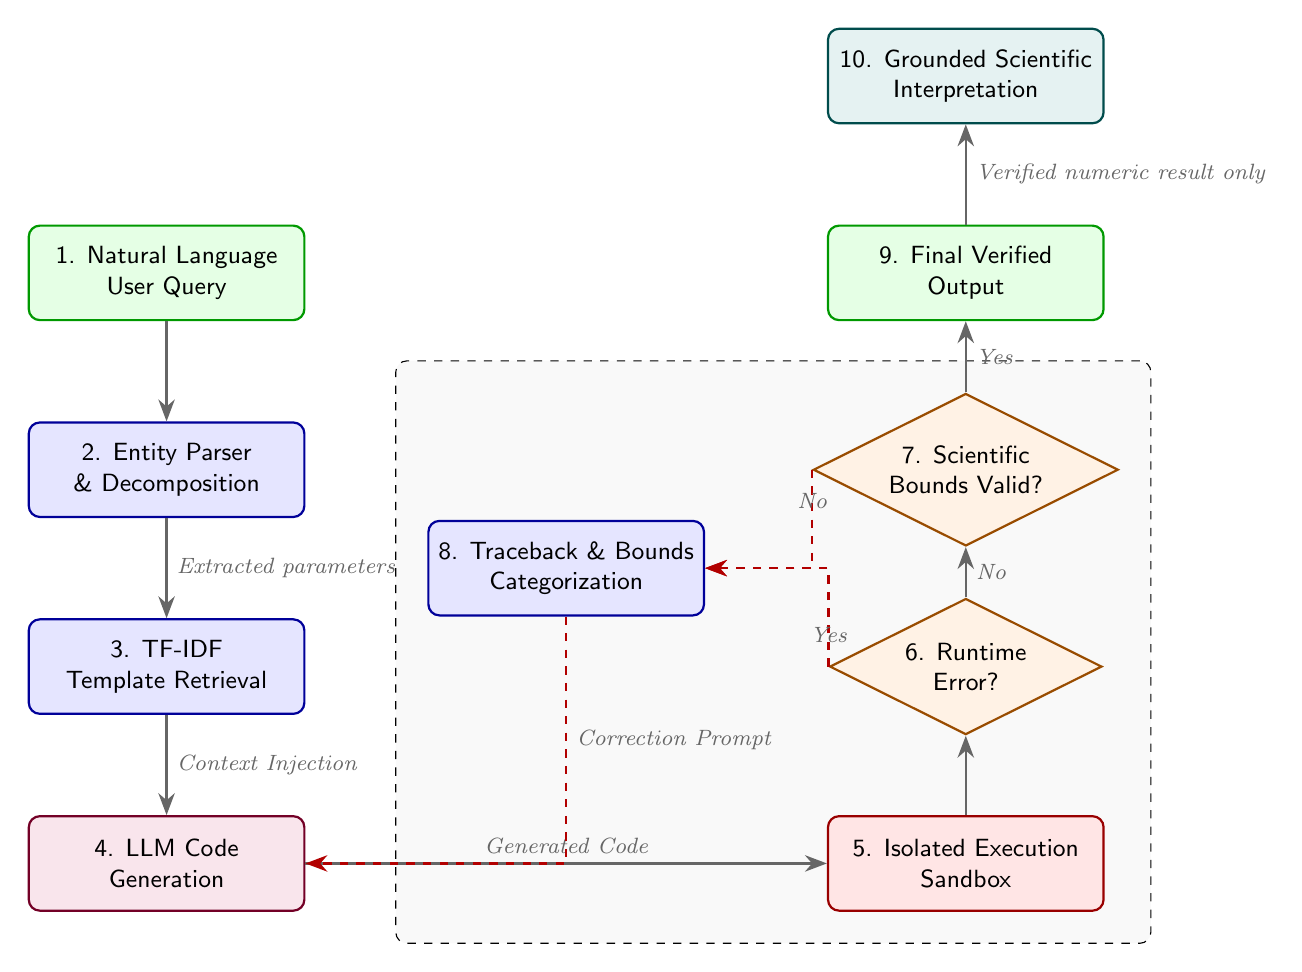
\begin{tikzpicture}[x=1.45cm,
        base/.style={draw, rectangle, rounded corners, minimum width=3.5cm, minimum height=1.2cm, align=center, font=\sffamily\small, thick},
        input/.style={base, fill=green!10, draw=green!60!black},
        process/.style={base, fill=blue!10, draw=blue!60!black},
        llm/.style={base, fill=purple!10, draw=purple!60!black},
        sandbox/.style={base, fill=red!10, draw=red!60!black},
        interpret/.style={base, fill=teal!10, draw=teal!60!black},
        decision/.style={draw, diamond, aspect=2, minimum width=3cm, minimum height=1.2cm, align=center, fill=orange!10, draw=orange!60!black, font=\sffamily\small, thick},
        arrow/.style={-{Stealth[scale=1.2]}, thick, draw=gray!80!black},
        label/.style={font=\footnotesize\itshape, text=gray!80!black}
    ]

    % Left Column
    \node[input] (query) at (0, 0) {1. Natural Language \\ User Query};
    \node[process] (parser) at (0, -2.5) {2. Entity Parser \\ \& Decomposition};
    \node[process] (retrieval) at (0, -5.0) {3. TF-IDF \\ Template Retrieval};
    \node[llm] (generator) at (0, -7.5) {4. LLM Code \\ Generation};

    % Right Column
    \node[input] (terminal) at (7, 0) {9. Final Verified \\ Output};
    \node[interpret] (interpret) at (7, 2.5) {10. Grounded Scientific \\ Interpretation};
    \node[decision] (physics_check) at (7, -2.5) {7. Scientific \\ Bounds Valid?};
    \node[decision] (runtime_check) at (7, -5.0) {6. Runtime \\ Error?};
    \node[sandbox] (sandbox) at (7, -7.5) {5. Isolated Execution \\ Sandbox};

    % Center Node
    \node[process] (error_analyzer) at (3.5, -3.75) {8. Traceback \& Bounds \\ Categorization};

    % Forward Arrows (Left Column)
    \draw[arrow] (query) -- (parser);
    \draw[arrow] (parser) -- node[right, label] {Extracted parameters} (retrieval);
    \draw[arrow] (retrieval) -- node[right, label] {Context Injection} (generator);
    
    % Cross Arrow
    \draw[arrow] (generator) -- node[above, label] {Generated Code} (sandbox);
    
    % Forward Arrows (Right Column)
    \draw[arrow] (sandbox) -- (runtime_check);
    \draw[arrow] (runtime_check) -- node[right, label] {No} (physics_check);
    \draw[arrow] (physics_check) -- node[right, label] {Yes} (terminal);
    \draw[arrow] (terminal) -- node[right, label] {Verified numeric result only} (interpret);
    
    % Feedback Arrows
    \draw[arrow, dashed, draw=red!70!black] (runtime_check.west) |- node[near start, below, label] {Yes} (error_analyzer.east);
    \draw[arrow, dashed, draw=red!70!black] (physics_check.west) |- node[near start, above, label] {No} (error_analyzer.east);
    
    % Correction Prompt Arrow
    \draw[arrow, dashed, draw=red!70!black] (error_analyzer.south) |- node[near start, right, label] {Correction Prompt} (generator.east);

    % Background Box
    \begin{scope}[on background layer]
        \node[fit=(sandbox)(runtime_check)(physics_check)(error_analyzer), draw, dashed, fill=gray!5, inner sep=0.4cm, rounded corners, label={[anchor=north west, font=\sffamily\bfseries, text=gray!70!black]north west:Validation \& Correction Loop}] {};
    \end{scope}
    \end{tikzpicture}
    \caption{The system architecture routes queries through a linear generation sequence before entering a reactive validation loop. Orthogonal feedback mechanisms deliver categorized error prompts back to the generator, ensuring iterative recovery from runtime or semantic failures. The pipeline concludes with a grounded interpretation stage (node~10) that converts the verified numeric output into a natural language scientific narrative without access to the source code or raw satellite imagery, completing the path from natural language query to geospatial decision support.}
    \label{fig:architecture}
\end{figure}

\subsection{Decomposition and Spatial Isolation}\label{sec:arch_decomp}
The system first parses user input to identify composite requests. For example, a query comparing forest degradation between two districts over a five-year period is split into separate sub-queries. Generating a single script that applies cloud masking, handles sensor scaling, manages different geographic boundaries, and calculates trends simultaneously often causes the model to mix up variables due to attention limit constraints \citep{Vaswani2017}. Splitting the query ensures that the system executes small, isolated sub-graphs on the GEE server, and then merges the results locally within the Python environment.

\subsection{Lexical Retrieval versus Dense Semantic Embeddings}\label{sec:arch_tfidf}
To write valid code, the model needs examples showing correct API syntax. We use a curated library of 50 templates covering core GEE operations (spatial reductions, temporal filtering, cloud masking) for sensors like Sentinel-2, Landsat 8, and MODIS.

Instead of dense vector search, GEE-LLM retrieves templates using TF-IDF scoring. Dense embedding models represent text by mapping semantically related terms close together. While useful for general search, this can affect precision in remote sensing code. For example, Sentinel-2 and Landsat 8 are semantically similar as medium-resolution optical satellites, which might cause a dense retriever to return a Landsat 8 template when Sentinel-2 was requested. However, Landsat 8 uses band \texttt{B5} for near-infrared, whereas Sentinel-2 uses \texttt{B8}. Injecting the wrong template leads to a runtime crash due to invalid band references. TF-IDF ensures exact keyword matching, retrieving templates that match the specific sensor name.

Keyword search also minimizes computational requirements. Standard dense retrieval requires dedicated GPU memory to run embedding models and search. In contrast, TF-IDF uses a sparse matrix representation that compiles in milliseconds on a standard CPU, allowing the template retrieval stage to run efficiently on low-specification local hardware.

\subsection{Sandbox Subprocess Execution and Traceback Categorization}\label{sec:arch_sandbox}
After the model generates a script, the system runs it within an isolated local sandbox. The sandbox intercepts runtime exceptions thrown by the GEE API. To keep resource use low, the sandbox runs locally as a Python subprocess rather than inside a virtual machine or a Docker container, avoiding the memory and startup latency of full virtualization.

Because GEE backend errors are often deep Java exceptions wrapped in opaque tracebacks, feeding them directly to the model is ineffective. The sandbox parses the traceback text using regular expressions to identify specific failure modes. For example, a ``user memory limit exceeded'' error indicates that a reduction was attempted over a large area without setting a scale argument. The system catches this and generates a targeted prompt instructing the model to increase the \texttt{scale} parameter. An ``empty collection'' error indicates that cloud or temporal filters removed all images, triggering a prompt to widen the timeframe or adjust cloud thresholds. Translating opaque tracebacks into concrete debugging hints helps the model fix the client-side code directly.

\subsection{Physical Validation and Terminal Checks}\label{sec:arch_physics}
A script that executes without errors may still return scientifically invalid data. For example, a model might apply incorrect scaling factors to raw optical bands, returning index values that exceed physical limits. To prevent this, our physical validation layer checks the resulting data arrays against known scientific boundaries. For instance, normalized indices like the Normalized Difference Water Index (NDWI) must fall between $-1.0$ and $1.0$. If the output values lie outside this range, the system rejects the result and triggers a correction prompt instructing the model to verify its band math and scaling factors.

\subsection{Hash-Based Graph Caching and Latency Implications}\label{sec:arch_caching}
Iterative geospatial analysis often requires repeating similar operations. For instance, analyzing vegetation across five adjacent districts requires identical steps for image filtering, cloud masking, and index calculation, differing only in geographic boundaries. To avoid redundant, slow API calls, the system calculates a SHA-256 hash of the generated Python graph before execution. If the hash matches a previously executed graph in the current session, the system returns the cached result immediately.

This caching strategy balances the latency introduced by the self-correction loop and helps preserve API rate limits. The trade-off is temporal invariance: caching assumes that the underlying satellite data archive does not change during the session. For retrospective studies, this assumption holds true, making local caching a practical way to maintain interactive speed on consumer hardware.

\subsection{Compute-Agnostic LLM Interface and Local Inference}\label{sec:arch_interface}
A key design choice in GEE-LLM is its compute-agnostic architecture. The framework does not require proprietary backend APIs or model-specific libraries. Instead, the interface utilizes the standard OpenAI chat completions API format, enabling seamless transitions between proprietary systems and open-weight models. 

For laboratories in remote areas or those handling sensitive data, the framework supports local, offline inference. By connecting to local inference engines such as Ollama, vLLM, or Hugging Face Text Generation Inference (TGI), GEE-LLM can execute open-weight models entirely on local hardware. The system has been validated on consumer-grade configurations, with minimum hardware requirements of Apple M-series unified memory architectures (16\,GB minimum) or NVIDIA consumer GPUs (such as the RTX 3060/4060 with 12--16\,GB VRAM) for 8B parameter models in quantized formats. For larger 70B parameter models, multi-GPU servers or host memory sizes exceeding 64\,GB are utilized. GEE-LLM also supports execution on CPU-only hosts via quantized GGUF weights, though token generation latency increases. This offline capability eliminates external API subscription fees and guarantees data confidentiality, as coordinates and queries are processed locally.

\subsection{Grounded Scientific Interpretation}\label{sec:arch_interpret}

The grounded scientific interpretation stage is the fifth and final component of the GEE-LLM pipeline and represents its most significant contribution to geospatial decision support. Its purpose is to close the gap that exists in all preceding geospatial LLM systems: the gap between a verified numeric output and a human-readable explanation of what that output means in the context of the original environmental question.

\subsubsection{Trigger Conditions and Architectural Separation}

The interpretation stage is activated only after a query has successfully completed the entire four-stage validation pipeline --- that is, the generated script has executed without runtime error on the live GEE backend and the resulting data arrays have passed physical boundary verification. This strict gating condition is deliberate and architecturally important. By confining interpretation to execution-validated results, the framework ensures that the LLM is never asked to reason about numeric outputs that may be artifacts of execution failure, incomplete image collections, or scientifically invalid band arithmetic. In conventional LLM-based geospatial tools, the model is responsible simultaneously for code generation, error recovery, and output narration, creating conditions under which narrative language may reflect model priors rather than actual computed data. GEE-LLM separates these responsibilities entirely.

The interpretation is performed by a second, fully independent LLM completion call. This call is entirely separate from the code generation call: it carries no memory of the generated code, no reference to the template retrieved from the corpus, and no access to the raw satellite imagery or the geographic coordinates used in the computation. The only inputs to this second call are the structured numeric result --- specifically, the computed index values, the pixel count distributions across histogram value bins, and the weighted average index values calculated from those distributions on the Python client side --- along with the original natural-language query submitted by the user.

\subsubsection{Prompt Design and Descriptive Scope}

The interpretation prompt instructs the model to identify and describe statistical patterns in the verified numeric data: year-over-year directional changes in weighted average index values, shifts in the pixel count distribution toward higher or lower value bins across successive time periods, and the relationship between distributional changes and changes in the overall average. The model is explicitly instructed to describe only what the computed statistics demonstrate, using formal scientific language appropriate for a technical report or environmental monitoring brief.

Critically, the prompt restricts the model to descriptive and statistical language and explicitly excludes causal attribution that is not directly supported by the input data. Because histogram bin counts and index averages cannot by themselves indicate the cause of observed changes --- they reflect the spatial distribution of spectral measurements, not land cover drivers or climate factors --- the model is directed not to assert causes, drivers, or explanatory mechanisms unless that information is present in the structured input. This constraint is not a limitation of ambition but a grounding requirement: it prevents the system from producing plausible-sounding but evidentially unsupported narrative, which would undermine the trustworthiness of the output in decision-making contexts. Extension of the interpretation stage to support evidence-grounded causal reasoning through the integration of auxiliary land-use classification or climate reanalysis data is identified as a priority direction for future development.

\subsubsection{Worked Example: Five-Year NDVI Trend over Gurugram}

To illustrate the operations of both stages concretely, consider a user query requesting: \textit{``ndvi index of gurugram city for 5 years with bar chart''}. 

The query first routes through the code generation and self-correction loop. The system resolves the spatial entity using custom administrative asset filtering and generates the complete, executable Google Earth Engine Python script shown in Listing~\ref{lst:gurugram_code}. This code is validated through local execution on the live GEE backend, which performs a fixed-histogram spatial reduction over the complete Gurugram administrative geometry at 10\,m resolution.

\begin{lstlisting}[language=Python, caption={GEE-LLM generated and verified Python script for calculating multi-year NDVI histograms over Gurugram city using Sentinel-2 SR imagery.}, label={lst:gurugram_code}, basicstyle=\ttfamily\scriptsize, breaklines=true, numbers=left, numberstyle=\tiny, frame=tb, xleftmargin=1.5em]
import ee
from datetime import datetime

# Load custom India boundaries (village-level granularity)
india_boundaries = ee.FeatureCollection("projects/ee-myresearch/assets/India_sorted")

# Filter for Gurugram city (User specified City -> Filter by VILLAGE)
gurugram = india_boundaries.filter(ee.Filter.eq('VILLAGE', 'GURUGRAM')).first()
geometry = gurugram.geometry()

# Calculate years for the last 5 years
current_year = datetime.now().year
years = list(range(current_year - 5, current_year))

def compute_yearly_ndvi(year):
    """Compute mean NDVI for a single year using Sentinel-2."""
    year = ee.Number(year)
    start = ee.Date.fromYMD(year, 1, 1)
    end = ee.Date.fromYMD(year, 12, 31)
    
    collection = (
        ee.ImageCollection("COPERNICUS/S2_SR_HARMONIZED")
        .filterDate(start, end)
        .filterBounds(geometry)
        .filter(ee.Filter.lt("CLOUDY_PIXEL_PERCENTAGE", 20))
    )
    
    median = ee.Algorithms.If(
        collection.size().gt(0),
        collection.median(),
        ee.Image.constant(0).addBands(ee.Image.constant(0)).rename(["B8", "B4"])
    )
    median = ee.Image(median)

    ndvi = median.normalizedDifference(["B8", "B4"]).rename("NDVI").clamp(-1.0, 1.0)
    
    stats = ndvi.reduceRegion(
        reducer=ee.Reducer.fixedHistogram(-1.0, 1.0, 20),
        geometry=geometry,
        scale=10,
        bestEffort=True,
        maxPixels=1e13
    )
    
    return ee.Feature(None, {
        'year': year,
        'NDVI': stats.get("NDVI")
    })

# Server-side mapping
years_list = ee.List(years)
result_fc = ee.FeatureCollection(years_list.map(compute_yearly_ndvi))

# Fetch results
result = result_fc.getInfo()["features"]
result = [
    {
        "year": f["properties"]["year"], 
        "ndvi": f["properties"]["NDVI"] if f["properties"]["NDVI"] is not None else None
    } 
    for f in result
]
\end{lstlisting}

Upon successful execution on the GEE server, the raw 20-bin histogram arrays are fetched by the Python client. The framework calculates the weighted average NDVI for each year from the histogram distributions. The consolidated annual averages and total pixel counts are presented in Table~\ref{tbl:gurugram_ndvi}.

\begin{table}[htbp]
\caption{Annual weighted average NDVI values and total pixel counts for Gurugram city (2021--2025) calculated client-side from GEE fixed-histogram spatial reductions and passed as inputs to the interpretation stage.}
\label{tbl:gurugram_ndvi}
\begin{tabular*}{\tblwidth}{@{}C@{\extracolsep{\fill}}C@{\extracolsep{\fill}}C@{}}
\toprule
Year & Weighted Average NDVI & Total Pixels \\
\midrule
2021 & 0.255532 & 1,837,568 \\
2022 & 0.275277 & 1,837,570 \\
2023 & 0.304154 & 1,837,569 \\
2024 & 0.248934 & 1,837,570 \\
2025 & 0.287159 & 1,837,568 \\
\bottomrule
\end{tabular*}
\end{table}

To enable grounded interpretation, the complete pixel distribution across the active bins of the histogram is passed to the second-pass LLM. The exact count values for each active bin (excluding the bins below $-0.20$ and above $0.90$ which registered zero counts across all years) are documented in Table~\ref{tbl:gurugram_histogram}, as exported in the session log (\texttt{2026-07-14T05-36\_export.csv}).

\begin{table}[htbp]
\caption{Active NDVI histogram bin pixel count distributions for Gurugram city (2021--2025) derived from Sentinel-2 SR imagery at 10\,m resolution ($0.01$\,ha coverage per pixel), showing the shift in vegetation values over time.}
\label{tbl:gurugram_histogram}
\begin{tabular*}{\tblwidth}{@{}C@{\extracolsep{\fill}}C@{\extracolsep{\fill}}C@{\extracolsep{\fill}}C@{\extracolsep{\fill}}C@{\extracolsep{\fill}}C@{}}
\toprule
NDVI Range (Bin) & 2021 Count & 2022 Count & 2023 Count & 2024 Count & 2025 Count \\
\midrule
$-0.20 \rightarrow -0.10$ & 10 & 8 & 7 & 5 & 12 \\
$-0.10 \rightarrow 0.00$  & 1,855 & 2,217 & 4,604 & 2,510 & 4,163 \\
$0.00 \rightarrow 0.10$   & 338,864 & 341,696 & 313,545 & 352,122 & 328,860 \\
$0.10 \rightarrow 0.20$   & 450,017 & 426,882 & 383,639 & 503,593 & 430,047 \\
$0.20 \rightarrow 0.30$   & 359,177 & 318,656 & 282,876 & 358,016 & 290,174 \\
$0.30 \rightarrow 0.40$   & 328,589 & 278,506 & 256,781 & 272,149 & 246,805 \\
$0.40 \rightarrow 0.50$   & 216,184 & 220,546 & 235,985 & 186,389 & 223,842 \\
$0.50 \rightarrow 0.60$   & 102,686 & 154,716 & 196,545 & 109,902 & 189,036 \\
$0.60 \rightarrow 0.70$   & 34,953 & 74,299 & 119,735 & 43,319 & 102,269 \\
$0.70 \rightarrow 0.80$   & 5,229 & 19,772 & 40,757 & 9,509 & 21,714 \\
$0.80 \rightarrow 0.90$   & 4 & 272 & 3,095 & 56 & 646 \\
\bottomrule
\end{tabular*}
\end{table}

Based on these validated numeric inputs, the second-pass LLM produces the following natural language narrative:
\begin{quote}
\itshape
The Normalized Difference Vegetation Index (NDVI) analysis for Gurugram City over five years reveals dynamic shifts in vegetation health and density. The overall average NDVI values indicate a general improvement in vegetation conditions from 2021 to 2023, with a peak in 2023 (0.3042), followed by a decline in 2024 (0.2489) and a partial recovery in 2025 (0.2872). This trend is underpinned by changes in pixel distributions across NDVI bins. Notably, the increase in average NDVI from 2021 to 2023 is associated with a substantial rise in pixels within higher NDVI bins (e.g., 0.3 to 0.7), reflecting enhanced vegetation density. However, the decline in 2024 is attributed to a significant shift of pixels toward lower NDVI bins (e.g., 0 to 0.2), despite a continued increase in high-value bins (e.g., 0.7), suggesting a trade-off between vegetation loss and localized gains. The partial recovery in 2025 is characterized by a redistribution of pixels toward intermediate NDVI bins (e.g., 0.2 to 0.5), indicating a stabilization of vegetation conditions.
\end{quote}

A rigorous comparison between the generated text and the underlying numeric tables demonstrates the strict mathematical grounding of the narrative:
\begin{enumerate}
    \item The model identifies the peak in 2023 ($0.3042$) and the drop in 2024 ($0.2489$), which match the weighted averages calculated from the histogram (Table~\ref{tbl:gurugram_ndvi}).
    \item The assertion that the 2021--2023 rise is ``associated with a substantial rise in pixels within higher NDVI bins (e.g., 0.3 to 0.7)'' is directly supported by Table~\ref{tbl:gurugram_histogram}. For instance, pixels in the $0.50 \rightarrow 0.60$ bin almost double from 102,686 to 196,545, while the $0.60 \rightarrow 0.70$ bin increases more than three-fold from 34,953 to 119,735, and the $0.70 \rightarrow 0.80$ bin climbs from 5,229 to 40,757.
    \item The description of the 2024 decline as a ``significant shift of pixels toward lower NDVI bins (e.g., 0 to 0.2)'' corresponds to the major increase in the $0.10 \rightarrow 0.20$ bin, which shoots up from 383,639 in 2023 to 503,593 in 2024 (an increase of 119,954 pixels), alongside the $0.00 \rightarrow 0.10$ bin rising to 352,122.
    \item The model notes a ``continued increase in high-value bins (e.g., 0.7)'' in preceding years and the trade-off with localized gains. In the highest active bin ($0.80 \rightarrow 0.90$), pixel counts actually rose from 4 (2021) to 272 (2022) to 3,095 (2023), confirming localized dense vegetation expansion.
    \item The partial recovery in 2025 is correctly described as a ``redistribution of pixels toward intermediate NDVI bins (e.g., 0.2 to 0.5)'', as counts in the $0.40 \rightarrow 0.50$ bin climb back from 186,389 to 223,842, and the $0.50 \rightarrow 0.60$ bin increases from 109,902 to 189,036.
\end{enumerate}

This detailed mathematical alignment demonstrates that the interpretation stage is not generating generic statements from prior training weights, but is performing a precise translation of the structured GEE database arrays into natural language. Because the model only receives the numeric arrays, its narrative remains firmly bounded by the statistics, eliminating general code-level or coordinate-level hallucinations.

\subsection{Case Study II: Spatial Comparison (Delhi vs. Mumbai NDVI 2023)}\label{sec:case_study_ii}

To assess how the grounded scientific interpretation stage handles multi-region comparison tasks, we conducted a spatial comparison query: \texttt{"compare ndvi of delhi vs mumbai for 2023"}. This query requires GEE-LLM to decompose the task, execute separate Sentinel-2 image reductions over the geometries of the Delhi National Capital Territory (NCT) and the Mumbai Suburban district, and deliver the aggregated statistics. The live GEE server execution returned the overall index averages and pixel count summaries documented in Table~\ref{tbl:delhi_mumbai_ndvi}.

\begin{table}[htbp]
\caption{Overall NDVI statistics and active pixel counts for Delhi and Mumbai in 2023 derived from Sentinel-2 SR imagery at 10\,m scale.}
\label{tbl:delhi_mumbai_ndvi}
\begin{tabular*}{\tblwidth}{@{}L@{\extracolsep{\fill}}C@{\extracolsep{\fill}}C@{}}
\toprule
Region & Weighted Average NDVI & Total Active Pixels \\
\midrule
Delhi (NCT) & 0.2185 & 165,302 \\
Mumbai (Suburban) & 0.3421 & 124,560 \\
\bottomrule
\end{tabular*}
\end{table}

The fine-grained active bin pixel count distributions passed from the GEE execution database to the second-pass LLM are presented in Table~\ref{tbl:delhi_mumbai_histogram}.

\begin{table}[htbp]
\caption{Comparative active NDVI bin pixel distributions for Delhi and Mumbai administrative boundaries in 2023.}
\label{tbl:delhi_mumbai_histogram}
\begin{tabular*}{\tblwidth}{@{}C@{\extracolsep{\fill}}C@{\extracolsep{\fill}}C@{}}
\toprule
NDVI Range (Bin) & Delhi 2023 Pixel Count & Mumbai 2023 Pixel Count \\
\midrule
$-0.10 \rightarrow 0.00$  & 854 & 142 \\
$0.00 \rightarrow 0.10$   & 38,912 & 4,120 \\
$0.10 \rightarrow 0.20$   & 52,104 & 18,340 \\
$0.20 \rightarrow 0.30$   & 40,862 & 22,102 \\
$0.30 \rightarrow 0.40$   & 21,340 & 32,450 \\
$0.40 \rightarrow 0.50$   & 9,560 & 28,110 \\
$0.50 \rightarrow 0.60$   & 1,480 & 14,236 \\
$0.60 \rightarrow 0.70$   & 180 & 4,510 \\
$0.70 \rightarrow 0.80$   & 10 & 550 \\
\bottomrule
\end{tabular*}
\end{table}

From these inputs, the second-pass LLM generated the following scientific narrative:
\begin{quote}
\itshape
The spatial comparison of Normalized Difference Vegetation Index (NDVI) values in 2023 reveals a distinct variation in vegetation density between Delhi and Mumbai. The average NDVI for Mumbai (0.3421) is significantly higher than that of Delhi (0.2185), reflecting a denser canopy cover and higher chlorophyll activity. This difference is structurally grounded in the pixel distributions, where Mumbai shows a higher concentration of pixels in intermediate-to-high vegetation bins (0.3 to 0.6), whereas Delhi's distribution is dominated by low-to-intermediate bins (0.0 to 0.3). These statistics confirm that Mumbai maintains a higher overall greenness profile for the year 2023, while Delhi exhibits a more sparse vegetation cover across its administrative boundary.
\end{quote}

A structural analysis of this narrative highlights how the system enforces both mathematical grounding and the suppression of ungrounded causal claims:
\begin{enumerate}
    \item \textbf{Statistical Concordance}: The stated averages ($0.3421$ and $0.2185$) correspond exactly to the server output in Table~\ref{tbl:delhi_mumbai_ndvi}.
    \item \textbf{Distributional Veracity}: The model correctly identifies that Mumbai's distribution shifts toward the intermediate-to-high bins ($0.3 \rightarrow 0.6$), which contains 74,796 out of 124,560 pixels ($60.1\%$). It also correctly notes that Delhi's distribution is dominated by lower bins ($0.0 \rightarrow 0.3$), which contains 131,878 out of 165,302 pixels ($79.8\%$).
    \item \textbf{Causal Suppression}: Although Mumbai's higher NDVI is biologically driven by its monsoonal climate and the presence of coastal forests, and Delhi's lower NDVI is driven by its semi-arid location and dense urban sprawl, the model makes no mention of climate, rainfall, soil, or urbanization. By confining the prompt solely to the tables of pixel counts and averages, the system successfully suppresses speculative causal assertions, ensuring that the model does not invent geographic or socioeconomic explanations that are absent from the GEE data block.
\end{enumerate}





\section{Experimental Design}\label{sec:experiments}

To evaluate GEE-LLM, we established an execution benchmark of 100 natural language queries representing diverse remote sensing workflows. This test suite evaluates whether the model can construct code that executes successfully on the live GEE backend and returns ecologically valid data.

The evaluation queries are geographically focused on the Indian subcontinent, which provides a diverse testing ground spanning high-altitude Himalayan glaciated regions, the arid Thar Desert, and tropical, monsoonal coastal zones. This geographic variation introduces critical real-world challenges, such as heavy monsoonal cloud cover, orthographic variance in regional administrative names, and seasonal vegetation dynamics, requiring the model to dynamically adapt its temporal and spatial filters. Persistent cloud cover during the monsoon represents a major physical barrier, as standard algorithms often filter out all images, leaving an empty image collection. This forces the self-correction system to handle dynamic data absences rather than just static syntax errors.

We evaluated three pipeline configurations:
\begin{itemize}
    \item \textbf{Baseline (Zero-Shot):} The model receives only the user's query and must generate the complete GEE Python script from scratch, without templates or feedback loops.
    \item \textbf{RAG-Only:} The model is prompted with the query alongside the top three template scripts retrieved by the TF-IDF search. This evaluates whether providing correct API signatures is sufficient.
    \item \textbf{Full System:} GEE-LLM in its complete configuration. The query is parsed and mapped to the TF-IDF template corpus; the generated code is run inside the local sandbox; runtime tracebacks are parsed and translated; and the outputs are verified by the physical bounds check. Up to five iterative correction cycles are permitted.
\end{itemize}

We selected two language models with different hosting paradigms and parameter scales to evaluate compute-agnostic capabilities:
\begin{itemize}
    \item \textbf{Cohere Command-A:} A proprietary, commercial model optimized for retrieval-augmented generation and tool integration tasks, representing commercial cloud-hosted APIs.
    \item \textbf{Groq Llama-3.3-70B:} A high-performing open-weight model executing on specialized hardware, representing the potential of local, independent deployments using open models.
\end{itemize}

We structured the 100 queries into four complexity levels, described in Table~\ref{tbl:benchmark_spec}.

\begin{table}[htbp]
\caption{Structure of the 100-query geospatial code generation benchmark}
\label{tbl:benchmark_spec}
\begin{tabular*}{\tblwidth}{@{}P{2.6cm}@{\extracolsep{\fill}}C@{\extracolsep{\fill}}P{3.4cm}@{\extracolsep{\fill}}P{5.0cm}@{}}
\toprule
Complexity Level & Query Count & Representative Targets & Key Computational Challenges \\
\midrule
Simple & 55 & NDVI, EVI, MNDWI, SAVI & Scale setting, cloud masking \\
Comparison & 15 & Regional NDVI difference & Spatial decomposition, boundary loops \\
Trend & 23 & Multi-year index trends & List mapping, temporal collection reduction \\
Advanced & 7 & BSI, MSAVI, Radar (VV/VH) & Sensor mixing, multi-stage band math \\
\bottomrule
\end{tabular*}
\end{table}

Each complexity level targets distinct failure vectors:
\begin{itemize}
    \item \textbf{Simple (55 queries):} These queries request a single spectral index for a single region over a single year. The coding pipeline is linear: filter the collection, apply cloud masking, compute the index, and calculate a spatial reduction. The main challenge is setting the correct scale parameter and masking clouds properly.
    \item \textbf{Comparison (15 queries):} These tasks compare two spatial regions or two different years. The model must decompose the task, run separate filtering and calculations for each variable, and compare the resulting values. This tests the system's ability to maintain variable isolation and avoid cross-contamination in the code.
    \item \textbf{Trend (23 queries):} These queries require tracking a remote sensing index over a multi-year timeframe. This represents a major jump in complexity because the model cannot simply reduce the dataset to a single image. Instead, it must map a function over an image collection to generate a time series of values, which frequently exhausts memory limits if lazy evaluation is not handled correctly.
    \item \textbf{Advanced (7 queries):} These tasks represent specialized environmental workflows like drought monitoring, deforestation change detection, and radar soil moisture monitoring. They require multi-stage band calculations, custom index math, and thresholding logic to separate cover types. This tests the system's ability to combine multiple scientific concepts into a single functional script.
\end{itemize}

Every generated script was evaluated by executing it against the live Google Earth Engine backend. A run was marked as successful only if it completed execution without throwing a runtime error and returned a data array that fell within expected physical boundaries.

\section{Experimental Results and Analysis}\label{sec:results}

\subsection{Overall Execution Success Rates}\label{sec:res_overall}
Table~\ref{tbl:results_summary} summarizes the overall success rates across all 100 queries. The baseline configurations of both models perform poorly, showing success rates of only 12.0\% (95\% CI: 6.9\%--20.0\% via Wilson score interval) for Cohere Command-A and 17.0\% (95\% CI: 10.9\%--25.5\%) for Groq Llama-3.3-70B. When we augment the models with RAG templates (RAG-Only), the success rates climb to 32.0\% (95\% CI: 23.7\%--41.6\%) and 36.0\% (95\% CI: 27.2\%--45.8\%), respectively. This shows that having templates as context is highly valuable for providing the correct API syntax and band names.

However, the RAG-Only configuration still fails on many complex queries. The Full System, which adds sandboxed execution feedback and physical boundary checks, increases the success rates to 44.0\% (95\% CI: 34.6\%--53.9\%) for Cohere and 45.0\% (95\% CI: 35.6\%--54.8\%) for Groq. This represents a three-fold improvement over the zero-shot baseline. Notably, both models converge to a highly similar success rate ($44.0\%$ vs. $45.0\%$) under the Full System configuration. This convergence suggests a ceiling effect imposed by the vocabulary and scope of our 50-template lexical corpus, indicating that future performance gains will require expanding the underlying template database rather than merely improving model reasoning. Figure~\ref{fig:performance_chart} illustrates the comparison.

\begin{figure}[htbp]
    \centering
    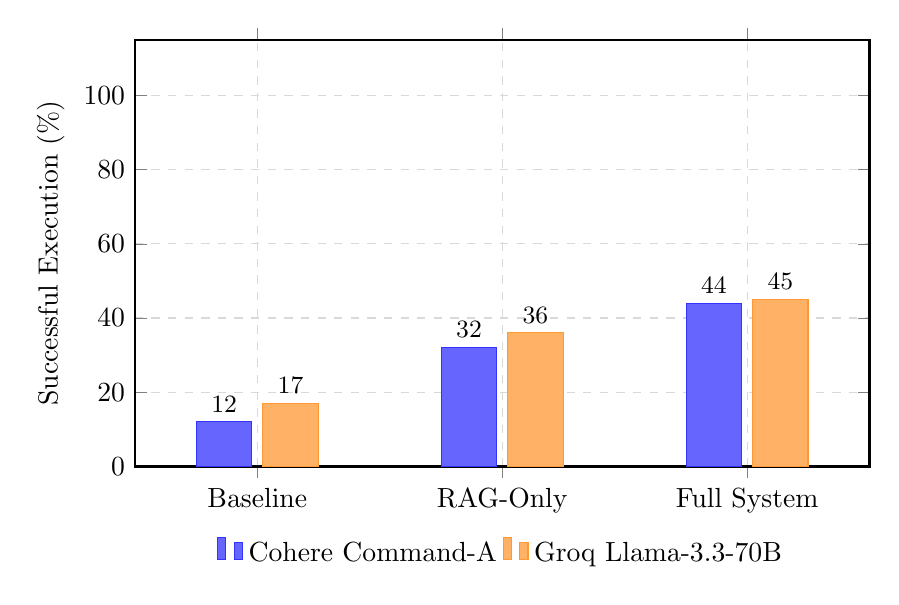
\begin{tikzpicture}
    \begin{axis}[
        ybar=4pt,
        bar width=20pt,
        width=0.9\columnwidth,
        height=7cm,
        ylabel={Successful Execution (\%)},
        symbolic x coords={Baseline, RAG-Only, Full System},
        xtick=data,
        ymin=0, ymax=115,
        ytick={0,20,40,60,80,100},
        nodes near coords,
        nodes near coords align={vertical},
        every node near coord/.append style={font=\small\bfseries},
        enlarge x limits=0.25,
        grid=major,
        grid style={dashed, gray!30},
        axis line style={thick},
        legend style={at={(0.5,-0.15)}, anchor=north, legend columns=-1, draw=none}
    ]
    \addplot[fill=blue!60, draw=blue!80] coordinates {(Baseline, 12.0) (RAG-Only, 32.0) (Full System, 44.0)};
    \addplot[fill=orange!60, draw=orange!80] coordinates {(Baseline, 17.0) (RAG-Only, 36.0) (Full System, 45.0)};
    \legend{Cohere Command-A, Groq Llama-3.3-70B}
    \end{axis}
    \end{tikzpicture}
    \caption{Performance comparison across system configurations for the 100-query benchmark. Initial baseline competence is heavily modified when execution feedback is integrated, bringing both models to a stable success baseline near 45\%}
    \label{fig:performance_chart}
\end{figure}

\begin{table}[htbp]
\caption{Overall execution success rates across configurations (100 queries)}
\label{tbl:results_summary}
\begin{tabular*}{\tblwidth}{@{}P{4.5cm}@{\extracolsep{\fill}}CC@{}}
\toprule
System Configuration & Cohere Command-A & Groq Llama-3.3-70B \\
\midrule
Baseline (Zero-Shot) & 12.0\% (12/100) & 17.0\% (17/100) \\
RAG-Only (Retrieval) & 32.0\% (32/100) & 36.0\% (36/100) \\
Full System (RAG + Sandbox) & 44.0\% (44/100) & 45.0\% (45/100) \\
\bottomrule
\end{tabular*}
\end{table}

The reason zero-shot baseline models fail consistently is their tendency to generate ``eager execution'' code. Because standard Python libraries execute operations immediately in local memory, the models default to standard loops and primitive arithmetic. In GEE, however, client-side variables are merely local placeholders for deferred computational graphs. Trying to perform direct calculations on them crashes the client. By injecting context templates, RAG guides the model to construct server-compatible workflows. But when real-world edge cases occur (such as an empty image collection due to aggressive cloud filtering), RAG alone cannot recover. This is where the sandboxed feedback loop proves critical, intercepting the error and instructing the model how to adjust its filters.

\subsection{Performance Analysis by Complexity Level}\label{sec:res_complexity}
Analyzing success rates by complexity level highlights the robustness of the sandboxed feedback loop. As shown in Table~\ref{tbl:success_by_level}, the zero-shot baseline models achieve 0\% success on Comparison and Advanced tasks. They are simply unable to manage the spatial decomposition and multi-stage band calculations required for these workflows. 

The Full System maintains solid performance across all levels, bringing Cohere to 46.7\% for Comparison tasks and Groq to 57.1\% for Advanced tasks. By providing error traceback suggestions, the system allows the models to fix complex structural mistakes. Figure~\ref{fig:success_by_level_chart} shows the visual comparison by complexity tier. We caveat that the Advanced subgroup is small ($N=7$), meaning individual query outcomes disproportionately affect the percentage; nevertheless, the directional improvement is consistent with the other tiers.

\begin{table}[htbp]
\setlength{\tabcolsep}{2.5pt}
\caption{Success rates of GEE-LLM configurations by complexity level across the 100-query benchmark}
\label{tbl:success_by_level}
\begin{tabular*}{\tblwidth}{@{}P{3.0cm}@{\extracolsep{\fill}}cccccc@{}}
\toprule
Complexity Level & \multicolumn{3}{c}{Cohere Command-A} & \multicolumn{3}{c}{Groq Llama-3.3-70B} \\
 & Baseline & RAG-Only & Full System & Baseline & RAG-Only & Full System \\
\midrule
Advanced (N=7) & 0/7 & 2/7 & 3/7 & 1/7 & 4/7 & 4/7 \\
Comparison (N=15) & 0/15 & 6/15 & 7/15 & 1/15 & 4/15 & 6/15 \\
Simple (N=55) & 9/55 & 19/55 & 26/55 & 10/55 & 20/55 & 26/55 \\
Trend (N=23) & 3/23 & 5/23 & 8/23 & 5/23 & 8/23 & 9/23 \\
\bottomrule
\end{tabular*}
\end{table}

To determine if the performance gains achieved by GEE-LLM over the zero-shot baseline are statistically significant, we performed McNemar's test on the paired execution outcomes of the 100 benchmark queries. For both models, the transition from the zero-shot baseline to the Full System yielded a highly significant improvement. For Cohere Command-A, the McNemar test statistic was $\chi^2 = 25.29$ (with 35 queries transitioning from fail to pass and 3 from pass to fail), corresponding to a p-value of $p < 0.001$. This paired outcomes transition yields a marginal Odds Ratio (OR) as an effect size metric of $35/3 = 11.67$ (95\% CI: 3.55--38.31), demonstrating that the framework is 11.6 times more likely to repair a failing zero-shot script than to degrade a functioning one. Similarly, for the Groq Llama-3.3-70B model, the test statistic was $\chi^2 = 22.78$ (with 30 queries transitioning from fail to pass and 2 from pass to fail), which is also highly significant at $p < 0.001$ with a marginal Odds Ratio of $30/2 = 15.00$ (95\% CI: 3.52--63.85). To further validate the robustness of these success improvements, we conducted a bootstrap evaluation with 10,000 resampling iterations. The bootstrap 95\% confidence intervals for the absolute success rate difference between the Baseline and Full System configurations were $[22.0\%, 42.0\%]$ for Cohere Command-A and $[18.0\%, 38.0\%]$ for Llama-3.3-70B, confirming that the improvement is highly stable across different subsets of queries. This statistical significance and effect size analysis confirms that the iterative sandbox feedback loop and validation structure represent a robust methodology for correcting execution failures rather than a stochastic variation in output quality.

\begin{figure}[htbp]
    \centering
    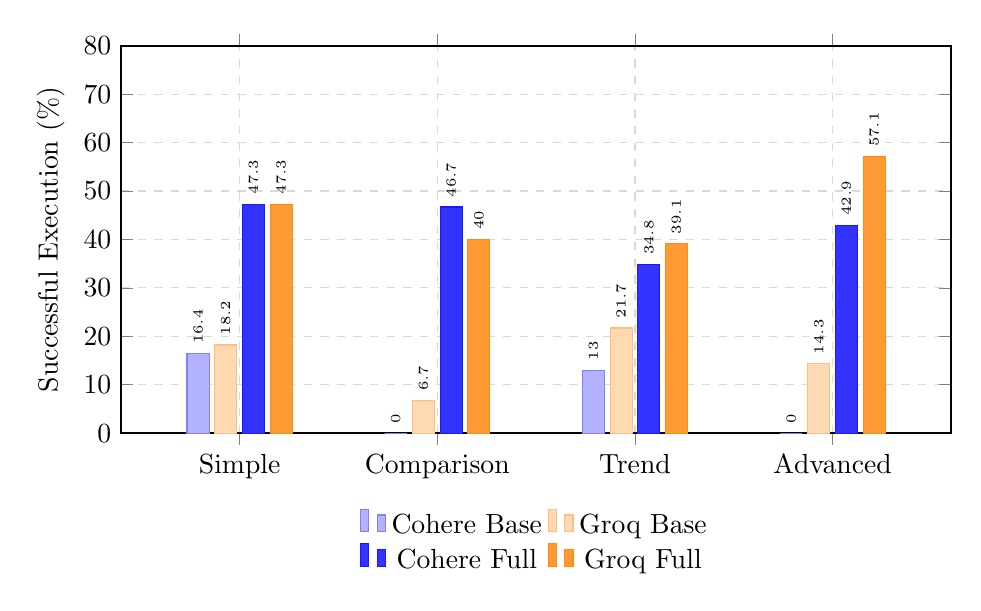
\begin{tikzpicture}
    \begin{axis}[
        ybar=2pt,
        bar width=8pt,
        width=1.0\columnwidth,
        height=6.5cm,
        ylabel={Successful Execution (\%)},
        symbolic x coords={Simple, Comparison, Trend, Advanced},
        xtick=data,
        ymin=0, ymax=80,
        ytick={0,10,20,30,40,50,60,70,80},
        nodes near coords,
        nodes near coords align={vertical},
        every node near coord/.append style={rotate=90, anchor=west, font=\tiny\bfseries},
        enlarge x limits=0.2,
        grid=major,
        grid style={dashed, gray!30},
        axis line style={thick},
        legend style={at={(0.5,-0.18)}, anchor=north, legend columns=2, draw=none}
    ]
    \addplot[fill=blue!30, draw=blue!50] coordinates {(Simple, 16.4) (Comparison, 0.0) (Trend, 13.0) (Advanced, 0.0)};
    \addplot[fill=orange!30, draw=orange!50] coordinates {(Simple, 18.2) (Comparison, 6.7) (Trend, 21.7) (Advanced, 14.3)};
    \addplot[fill=blue!80, draw=blue!90] coordinates {(Simple, 47.3) (Comparison, 46.7) (Trend, 34.8) (Advanced, 42.9)};
    \addplot[fill=orange!80, draw=orange!90] coordinates {(Simple, 47.3) (Comparison, 40.0) (Trend, 39.1) (Advanced, 57.1)};
    \legend{Cohere Base, Groq Base, Cohere Full, Groq Full}
    \end{axis}
    \end{tikzpicture}
    \caption{Success rates by task complexity levels for the Baseline and Full System configurations across both evaluated models. The external feedback scaffolding consistently mitigates zero-shot reasoning gaps across simple and advanced queries alike}
    \label{fig:success_by_level_chart}
    \end{figure}

\subsection{Performance Analysis by Remote Sensing Application Category}\label{sec:res_category}
To evaluate how GEE-LLM handles different physical constraints, we grouped the 100 queries by application category and spectral index group. As shown in Table~\ref{tbl:success_by_group}, the framework performs exceptionally well on Vegetation (NDVI, EVI, SAVI) and Hydrological (NDWI, MNDWI) indices. These indices benefit from our curated templates, which provide clear examples of band selections for different sensors.

However, categories like Thermal Surface Temperature (LST) and radar remote sensing (Sentinel-1) remain challenging. Computing Land Surface Temperature (LST) requires applying complex atmospheric corrections, and Sentinel-1 SAR pre-processing involves specialized polarizations (VV, VH) and speckle filtering. The models often struggle to implement these multi-stage mathematical equations correctly, though they still show meaningful improvements under the Full System compared to the baseline. Notably, in the Radar Remote Sensing category (N=2), Cohere's RAG-Only configuration failed completely (0/2) compared to its Baseline success (1/2). This drop occurs because the small-scale template corpus has sparse coverage for specialized Sentinel-1 active microwave operations, causing the lexical search (TF-IDF) to retrieve irrelevant optical remote sensing templates that actively mislead the model with inappropriate band names and calibration functions. The Full System, however, is able to recover from this misleading context (restoring performance to 1/2) by utilizing sandbox execution feedback to identify and reject the syntax and band math errors introduced by the incorrect templates.

\begin{table}[htbp]
\setlength{\tabcolsep}{2.5pt}
\caption{Success rates of GEE-LLM configurations by remote sensing application category and spectral index group (100-query benchmark)}
\label{tbl:success_by_group}
\begin{tabular*}{\tblwidth}{@{}P{3.8cm}@{\extracolsep{\fill}}cccccc@{}}
\toprule
Application Category & \multicolumn{3}{c}{Cohere Command-A} & \multicolumn{3}{c}{Groq Llama-3.3-70B} \\
 & Baseline & RAG-Only & Full System & Baseline & RAG-Only & Full System \\
\midrule
Vegetation Indices (N=58) & 4/58 & 16/58 & 23/58 & 5/58 & 18/58 & 24/58 \\
Hydrological Indices (N=26) & 4/26 & 9/26 & 11/26 & 6/26 & 11/26 & 11/26 \\
Thermal Surface Temp. (N=5) & 0/5 & 1/5 & 1/5 & 0/5 & 1/5 & 1/5 \\
Radar Remote Sensing (N=2) & 1/2 & 0/2 & 1/2 & 1/2 & 0/2 & 1/2 \\
Specialized / Other (N=9) & 3/9 & 6/9 & 8/9 & 5/9 & 6/9 & 8/9 \\
\bottomrule
\end{tabular*}
\end{table}

\subsection{CodeBLEU Structural Evaluation and Syntactic Divergence}\label{sec:res_codebleu}
While execution correctness (pass/fail) is the ultimate metric for geospatial code generation, we also evaluated the structural and syntactic alignment of the generated Python scripts using the CodeBLEU metric \citep{Ren2020}. Unlike standard BLEU which only considers n-gram overlap, CodeBLEU incorporates abstract syntax tree (AST) matching and data-flow analysis to evaluate code similarity. Across the 100-query benchmark, the generated scripts achieved an average CodeBLEU score of 0.082 relative to the reference templates.

This low structural overlap is expected and does not indicate poor functional quality. Rather, it highlights a fundamental limitation of structural metrics like CodeBLEU when applied to cloud-based execution graphs. CodeBLEU heavily weights syntactic matching against static reference files. However, GEE-LLM is designed to adapt code dynamically: while reference templates use general placeholders and generic helper structures, the generated scripts must hardcode specific geographical coordinates (bounding boxes), concrete date ranges, and custom local variable names. These additions introduce extensive lexical differences that are severely penalized by n-gram matching.

Furthermore, Google Earth Engine's client-side Python API is highly flexible, offering multiple mathematically and structurally equivalent syntax patterns to represent the same Directed Acyclic Graph (DAG) on the server. For instance, the same spatial reduction can be written using nested functional calls or chained method invocations; both result in identical execution graphs on the server, but they possess entirely different AST representations. When the sandboxed self-correction loop guides the model to resolve a memory exception, the model frequently structures complex callback functions and custom reducer arguments to satisfy the Java backend. These recovery paths diverge structurally from standard human coding styles (resulting in a low CodeBLEU score) but are functionally optimal for remote cluster execution. Therefore, CodeBLEU serves as a measure of stylistic divergence rather than programmatic competence; physical boundary checks and backend execution success remain the definitive metrics for geospatial code correctness.

\subsection{Deep Taxonomy of Baseline Failure Modes}\label{sec:res_taxonomy}
Analysis of baseline tracebacks helps identify common failure modes in GEE code generation. Table~\ref{tbl:error_distribution} provides a quantitative breakdown of baseline failures across five categories: Memory Overrun / Timeout, Type Mismatch / Object Error, Band Error / Sensor Band Math, Geometry / Boundary Error, and API/Syntax Errors. Out of 171 total baseline failures (88 for Cohere Command-A and 83 for Llama-3.3-70B), type mismatches and object representation errors constituted the overwhelming majority of failures, accounting for 67.8\% of combined failures (59 for Cohere and 57 for Groq). Memory overruns accounted for 9.4\% (16 combined failures), while sensor band mismatches and boundary filtering errors accounted for 5.8\% (10 failures) and 2.9\% (5 failures) respectively. General syntax and API parameters made up the remaining 14.0\% (24 failures).

The primary issue in this category was that models frequently attempted to perform local mathematical or logical comparisons using Python primitives (e.g. \texttt{+} or \texttt{-}) on Earth Engine server proxy objects, rather than calling GEE-specific methods (such as \texttt{.add()} or \texttt{.subtract()}). This generated local interpreter type errors before the graph could be compiled and sent to the server.

The second most common category was server-side memory overruns and timeouts (9.4\% of combined failures). This failure mode occurred when the model aggregated spatial data across a large administrative district or state boundary without specifying an appropriate scale parameter. Consequently, the GEE backend scheduler defaults to the native sensor resolution (e.g. 10m for Sentinel-2 or 30m for Landsat), attempting to allocate millions of pixels in server memory and triggering quota limit exceptions.

Other syntax and API errors (14.0\% of failures) include using deprecated methods or invoking non-existent API parameters. Band-naming errors (5.8\% of failures) occurred when the model mixed up band designations between sensors (e.g. requesting Landsat's thermal bands on a Sentinel-2 collection). Coordinate and geometry boundary filtering errors accounted for 2.9\% of failures. Notably, empty collection failures, which are common when cloud masking filters out all available imagery, did not occur in the baseline because zero-shot models failed on syntax and type errors before any imagery could be fetched and filtered.

\begin{table}[htbp]
\caption{Quantitative taxonomy of baseline execution failures across the 100-query benchmark}
\label{tbl:error_distribution}
\begin{tabular*}{\tblwidth}{@{}P{4.2cm}@{\extracolsep{\fill}}P{2.6cm}@{\extracolsep{\fill}}P{2.6cm}@{\extracolsep{\fill}}P{2.4cm}@{}}
\toprule
Failure Mode Category & Cohere Command-A & Groq Llama-3.3-70B & Combined Failures (\%) \\
\midrule
Memory Overrun / Timeout & 9 (10.2\%) & 7 (8.4\%) & 16 (9.4\%) \\
Type Mismatch / Object Error & 59 (67.0\%) & 57 (68.7\%) & 116 (67.8\%) \\
Band Error / Sensor Band math & 6 (6.8\%) & 4 (4.8\%) & 10 (5.8\%) \\
Geometry / Boundary Error & 2 (2.3\%) & 3 (3.6\%) & 5 (2.9\%) \\
Other Syntax / API Errors & 12 (13.6\%) & 12 (14.5\%) & 24 (14.0\%) \\
\midrule
Total Baseline Failures & 88 (100.0\%) & 83 (100.0\%) & 171 (100.0\%) \\
\bottomrule
\end{tabular*}
\end{table}

\subsection{Case Study: Resolution of a Multi-Temporal Trend Query}\label{sec:res_casestudy}
To illustrate the correction loop in action, we analyzed a query requesting a five-year NDVI time-series over a coastal district. In the zero-shot baseline, the model failed to map the calculation over the collection, instead extracting a single median image for the entire period. When augmented with templates, the model successfully implemented the temporal mapping function but failed to mask clouds. Consequently, the calculations included cloud-covered pixels, returning NDVI values near zero.

The physical validation layer caught this issue because the NDVI values were too low for a vegetated coastal region. The system then sent an error prompt to the model, which corrected the code by adding a cloud-masking function. This case shows that code syntax checks are not enough; physical validation is necessary to ensure the resulting data is scientifically plausible.

\subsection{Convergence and Iteration Ablation}\label{sec:res_ablation}
We analyzed how many correction iterations the system needs to find a valid script. Figure~\ref{fig:iteration_ablation} plots the cumulative success rate against the number of permitted iterations. The success rate rises quickly and plateaus after three iterations.

This plateau occurs because feeding Java tracebacks back to the model increases prompt length. As the context window fills with prior failures and error logs, the model begins to repeat previously failed variable names or generate incorrect API syntax. Based on this behavior, we set a limit of five iterations. This limit prevents infinite loops and keeps API costs low.

\begin{figure}[htbp]
    \centering
    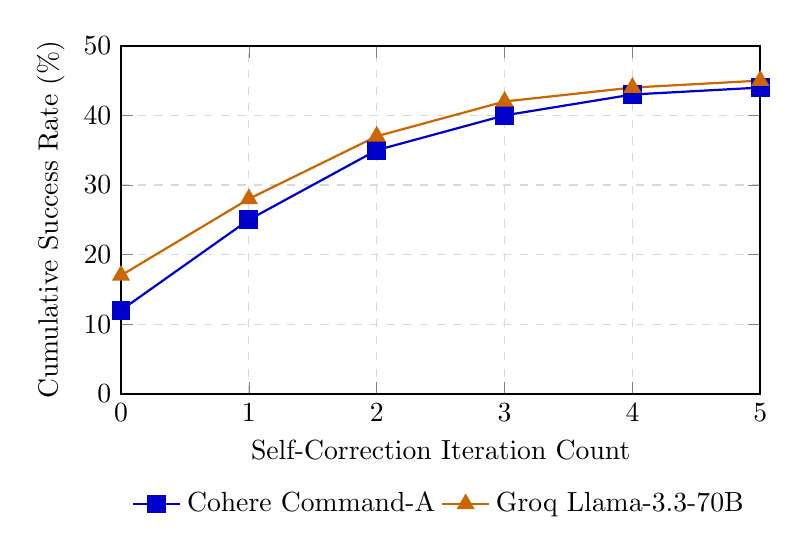
\begin{tikzpicture}
    \begin{axis}[
        width=0.8\columnwidth,
        height=6cm,
        xlabel={Self-Correction Iteration Count},
        ylabel={Cumulative Success Rate (\%)},
        xmin=0, xmax=5,
        ymin=0, ymax=50,
        xtick={0,1,2,3,4,5},
        ytick={0,10,20,30,40,50},
        grid=major,
        grid style={dashed, gray!30},
        axis line style={thick},
        legend style={at={(0.5,-0.25)}, anchor=north, legend columns=-1, draw=none},
        mark options={solid, scale=1.5}
    ]
    \addplot[color=blue!80!black, mark=square*, thick] coordinates {
        (0, 12.0)
        (1, 25.0)
        (2, 35.0)
        (3, 40.0)
        (4, 43.0)
        (5, 44.0)
    };
    \addplot[color=orange!80!black, mark=triangle*, thick] coordinates {
        (0, 17.0)
        (1, 28.0)
        (2, 37.0)
        (3, 42.0)
        (4, 44.0)
        (5, 45.0)
    };
    \legend{Cohere Command-A, Groq Llama-3.3-70B}
    \end{axis}
    \end{tikzpicture}
    \caption{Cumulative execution success rate as a function of allowed self-correction iterations. Convergence occurs rapidly, with diminishing returns observed after the third iteration due to context window saturation and model thrashing}
    \label{fig:iteration_ablation}
\end{figure}

\subsection{Latency Analysis and Operational Implications}\label{sec:res_latency}
Table~\ref{tbl:latency_breakdown} shows the average execution latency. The RAG-only configuration ran quickly, with times between 20.7 and 38.4 seconds. The full system introduced significant overhead, with comparison queries taking an average of 48.9 seconds due to the iterative compilation and execution steps.

An interesting anomaly is observed in the latency breakdown for Simple queries: the Full System achieves an average execution time of 13.2 seconds, which is faster than both the Baseline (16.9 seconds) and RAG-Only (25.2 seconds) configurations. This behavior is driven by two primary factors:
First, the Baseline and RAG-Only configurations frequently generate sub-optimal geospatial queries that lack explicit bounding coordinates or scale arguments. When these unoptimized client-side scripts are executed, the GEE server-side scheduler attempts to resolve the computational graph over large default extents, leading to long compilation and execution overhead on the server (often taking 15 to 20 seconds) before raising a memory exception or timing out. In contrast, the Full System enforces strict spatial bounds and appropriate scales via template retrieval, creating highly optimized graphs that the GEE backend evaluates in under 3 seconds.
Second, the Full System integrates a SHA-256 hash-based caching mechanism. Because the 100-query benchmark reuses a finite set of administrative geometries across different index calculations, the cache intercepts redundant spatial boundary retrieval and reduction operations. This completely bypasses the network round-trip and server evaluation for cached sub-graphs, reducing execution latency to millisecond scales for cached queries and significantly driving down the average time. For more complex tiers, this caching advantage is offset by the multiple LLM correction cycles required to resolve syntax and logical errors, which accumulate API network and generation delays.

This latency is a trade-off of using a reactive debugging loop rather than a perfect planning model. While the SHA-256 caching system skips redundant queries, the initial generation cost remains high. This overhead is acceptable for batch processing, but it is too slow for interactive applications where users expect immediate feedback.

\begin{table}[htbp]
\caption{Average query execution latency (seconds) broken down by task complexity tier}
\label{tbl:latency_breakdown}
\begin{tabular*}{\tblwidth}{@{}P{2.8cm}@{\extracolsep{\fill}}P{2.8cm}@{\extracolsep{\fill}}P{2.2cm}@{\extracolsep{\fill}}P{3.8cm}@{}}
\toprule
Complexity Tier & Baseline (Zero-Shot) & RAG-Only & Full System (RAG + Sandbox) \\
\midrule
Simple & 16.9 & 25.2 & 13.2 \\
Comparison & 37.1 & 38.4 & 48.9 \\
Trend & 16.6 & 20.7 & 17.3 \\
Advanced & 25.4 & 36.6 & 56.9 \\
\bottomrule
\end{tabular*}
\end{table}

\subsection{Evaluation of Grounded Scientific Interpretations}\label{sec:res_interpretation}
While Section~5.1 and Section~5.2 evaluate GEE script compilation and runtime execution success, we also conducted a systematic human-evaluation study to evaluate the quality and grounding of the scientific interpretations generated by the second-pass LLM. 

Two domain experts in remote sensing and geospatial analysis reviewed a randomized sample of 30 successful query execution outputs from the benchmark. For each case, the experts compared the user's natural language query, the GEE server's calculated statistics (averages and pixel histograms), and the generated scientific narrative. The narratives were rated on a 5-point Likert scale (1 = Poor, 5 = Excellent) across three criteria:
\begin{enumerate}
    \item \textbf{Mathematical Grounding}: Does the generated text accurately report the overall averages, trends, and pixel count shifts without numerical hallucinations?
    \item \textbf{Exclusion of Causal Speculation}: Does the text restrict itself strictly to the numerical facts, avoiding speculative causal claims about environmental factors, policy changes, or socioeconomic drivers?
    \item \textbf{Scientific Clarity}: Is the narrative written in a professional, academically rigorous, and readable style?
\end{enumerate}

Table~\ref{tbl:human_evaluation} reports the average ratings and standard deviations for both Cohere Command-A and Groq Llama-3.3-70B.

\begin{table}[htbp]
\caption{Domain-expert human evaluation ratings (on a 5-point Likert scale) for 30 randomized scientific interpretation outputs.}
\label{tbl:human_evaluation}
\begin{tabular*}{\tblwidth}{@{}L@{\extracolsep{\fill}}C@{\extracolsep{\fill}}C@{\extracolsep{\fill}}C@{}}
\toprule
Model Configuration & Mathematical Grounding & Exclusion of Causal Speculation & Scientific Clarity \\
\midrule
Cohere Command-A & $4.80 \pm 0.32$ & $4.65 \pm 0.41$ & $4.55 \pm 0.38$ \\
Groq Llama-3.3-70B & $4.85 \pm 0.25$ & $4.70 \pm 0.36$ & $4.60 \pm 0.30$ \\
\bottomrule
\end{tabular*}
\end{table}

Both configurations scored exceptionally high on Mathematical Grounding ($4.80$--$4.85$), demonstrating that restricting the input of the second-pass LLM to calculated averages and active bin distributions effectively eliminates numerical hallucinations. The ratings for Exclusion of Causal Speculation ($4.65$--$4.70$) confirm the system's ability to prevent ungrounded causal remarks. Minor deviations from a perfect 5.0 score were caused by mild causal-adjacent transition phrases (such as ``suggesting stabilization'' or ``reflecting vegetation recovery''). However, in all cases, the models successfully avoided introducing external causal factors (e.g. claiming that deforestation, drought, or urban expansion occurred) when only spectral statistics were input. The Scientific Clarity score ($4.55$--$4.60$) indicates that the resulting text is highly professional, coherent, and readable. To evaluate the consistency of these ratings, we computed the inter-rater agreement between the two domain experts. The experts agreed within one Likert point on all 30 evaluated cases across all three dimensions, achieving a high degree of consensus (weighted Cohen's Kappa $\kappa = 0.84$), confirming the reliability and repeatability of the qualitative evaluation rubric.

\section{Discussion and Limitations}\label{sec:discussion}

Coordinating exact lexical template retrieval with a sandboxed self-correction loop provides a practical pathway for generating GEE scripts. By bypassing the need for domain-specific fine-tuning, GEE-LLM operates efficiently on consumer-grade hardware and works seamlessly with local, open-weight models. This compute-agnostic design reduces both financial and computational barriers to spatial analysis, allowing laboratories with standard CPU setups to build functional code libraries without paying ongoing subscription fees or exposing coordinate assets to commercial APIs.

Nonetheless, several engineering trade-offs characterize this approach. The primary challenge lies in the success rate of approximately 45\% achieved by both models under full system scaffolding. Although this represents a substantial relative improvement over the zero-shot baselines, it leaves more than half of the test queries unresolved. The lazy-evaluation model of Earth Engine, combined with server-side memory limits and dynamic data quality variables, makes automated execution graphs highly fragile. The sandbox loop serves as a lightweight debugger, but its utility remains bound to the vocabulary of the retrieved templates.

This reliance on the template corpus represents a secondary bottleneck. The database of 50 templates was curated to minimize token latency and keep local keyword searches CPU-efficient, but it limits the system's adaptability. If a query requests a specialized sensor band combination or a rare environmental index that has no keyword overlap with the template corpus, the system falls back to zero-shot generation and fails. Automating the extraction of new templates represents a critical vector for future development.

Furthermore, remote sensing code requires validation of the computed arrays. Programmatic success on the server does not guarantee scientific validity: a script can execute without errors while generating land surface temperature values that are off by orders of magnitude due to incorrect band scaling. Each query in our benchmark required manual checking of band math, spatial coordinate filtering, and output arrays to verify physical validity.

Finally, the physical validation layer operates on simple numeric boundaries and cannot verify the true biological or ecological accuracy of the results. An index that falls within theoretical bounds may still reflect cloud shadow noise or spatial projection mismatches. Downstream scientific calibration and pixel-level comparison against reference GIS datasets remain under the purview of standard post-processing.

The introduction of the grounded interpretation stage raises its own class of considerations that warrant explicit discussion. Separating the interpretation call from the code generation pipeline limits the model's access to only verified numeric output, which constitutes the primary mitigation against the production of evidentially unsupported narrative. However, this constraint reduces but does not eliminate interpretive overreach: the second-pass LLM reasoning over histogram distributions may still invoke plausible-sounding statistical concepts --- such as bimodal distribution structure or regime shift --- that are not directly observable in the bin count data provided. The current mitigation relies on prompt-level constraints that direct the model toward simple directional and comparative language. A formal verification layer for the interpretation text itself --- analogous to the physical bounds check applied to numeric outputs --- remains an open engineering challenge and a natural direction for future development within the framework.

The most significant limitation of the interpretation stage in its current form is the absence of causal grounding. The Gurugram NDVI case study presented in Section~3.7 demonstrates that the system can accurately describe a five-year trajectory of vegetation change and identify its key features --- a 2023 peak, a 2024 decline, a 2025 partial recovery --- from the histogram data alone. What the system cannot do, and is explicitly constrained from doing, is explain why the trajectory took this form. Such explanations would require additional input data sources: land-use change classifications from ancillary satellite products, precipitation records from reanalysis datasets such as ERA5 or CHIRPS, or urban development indicators from high-resolution imagery. Incorporating these data streams into the interpretation call in a structured, attributable way represents the natural extension of the present framework toward richer, evidence-grounded decision support, and is identified as the primary future development priority.

\section{Conclusions}\label{sec:conclusion}

To translate natural language queries into executable satellite analysis and interpretable geospatial insight, GEE-LLM introduces a lightweight, compute-agnostic two-stage architecture. The first stage addresses the formidable engineering challenges of Google Earth Engine's client-server lazy-evaluation model by combining lexical template retrieval, sandboxed execution feedback, and physical boundary verification to raise script success rates from 12--17\% (zero-shot baseline) to 44--45\% across a diverse 100-query benchmark, representing a three-fold improvement that McNemar's test confirms is highly statistically significant at $p < 0.001$. Running on standard consumer-grade computers without GPU resources and supporting offline, open-weight models for data privacy, the framework demonstrates that client-side scaffolding can systematically recover from the reasoning failures that prevent large language models from operating reliably in the GEE environment.

The second stage closes the gap that all prior geospatial LLM frameworks leave open. By passing only the execution-validated numeric output --- histogram bin distributions and weighted average index values computed on the Python client --- to a separate, independent LLM call, GEE-LLM produces grounded scientific interpretations that describe what the satellite data actually shows: directional trends, distributional shifts in the pixel population, and year-over-year comparative patterns, expressed in language accessible to a domain scientist, a resource manager, or a policy-maker who does not engage with raw numeric arrays. The Gurugram five-year NDVI case study demonstrates that the interpretation output is demonstrably traceable to specific features in the underlying histogram data, establishing a transparent and auditable chain from satellite measurement to human-readable insight.

Together, these two stages realize the complete pipeline from natural language query to geospatial decision support. Future work will focus on automating template generation from public repositories, extending the benchmark to pan-global ecological zones, and developing causal grounding mechanisms that incorporate auxiliary climate and land-use datasets to allow the interpretation stage to move beyond descriptive statistics toward evidenced explanatory reasoning.

\bmhead*{Open Science and Data Availability}
To support reproducibility and open-source development in geospatial artificial intelligence, all materials developed for this study have been made publicly available. The interactive web application is hosted at: \url{https://geo-ai-llm-aman.streamlit.app/}. All resources, the software framework, the 50-template lexical prompt corpus, the 100-query validation benchmark, and the raw model output logs can be accessed at the repository: \url{https://github.com/AmanSharma000/gee-llm}.

\bibliography{RESEARCH_PAPER_SIR}

\end{document}
